\section{Performance}

\subsection{Module testing (QA, full chain, r/a sources, beam)}

\begin{figure}[hbt] 
\centering 
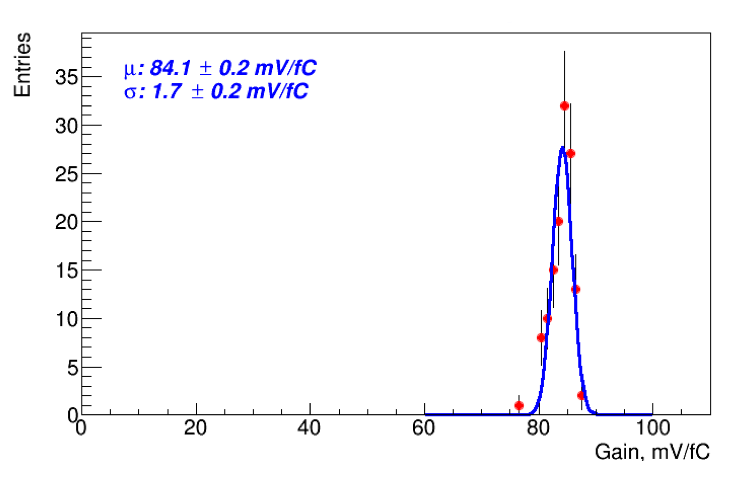
\includegraphics[width=0.5\columnwidth,keepaspectratio]{gain-chip.png}
\caption{Gain vs. channel.}
\label{fig:gain-chip}
\end{figure}

\begin{figure}[hbt] 
\centering 
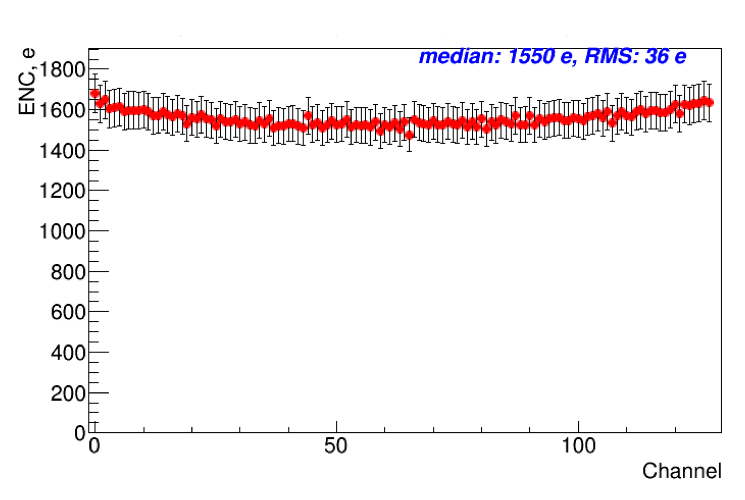
\includegraphics[width=0.5\columnwidth,keepaspectratio]{enc-chip.png}
\caption{Equivalent Noise Charge vs. channel.}
\label{fig:enc-chip}
\end{figure}

\subsection{Integration and system checkout}

\begin{figure}[hbt] 
\centering 
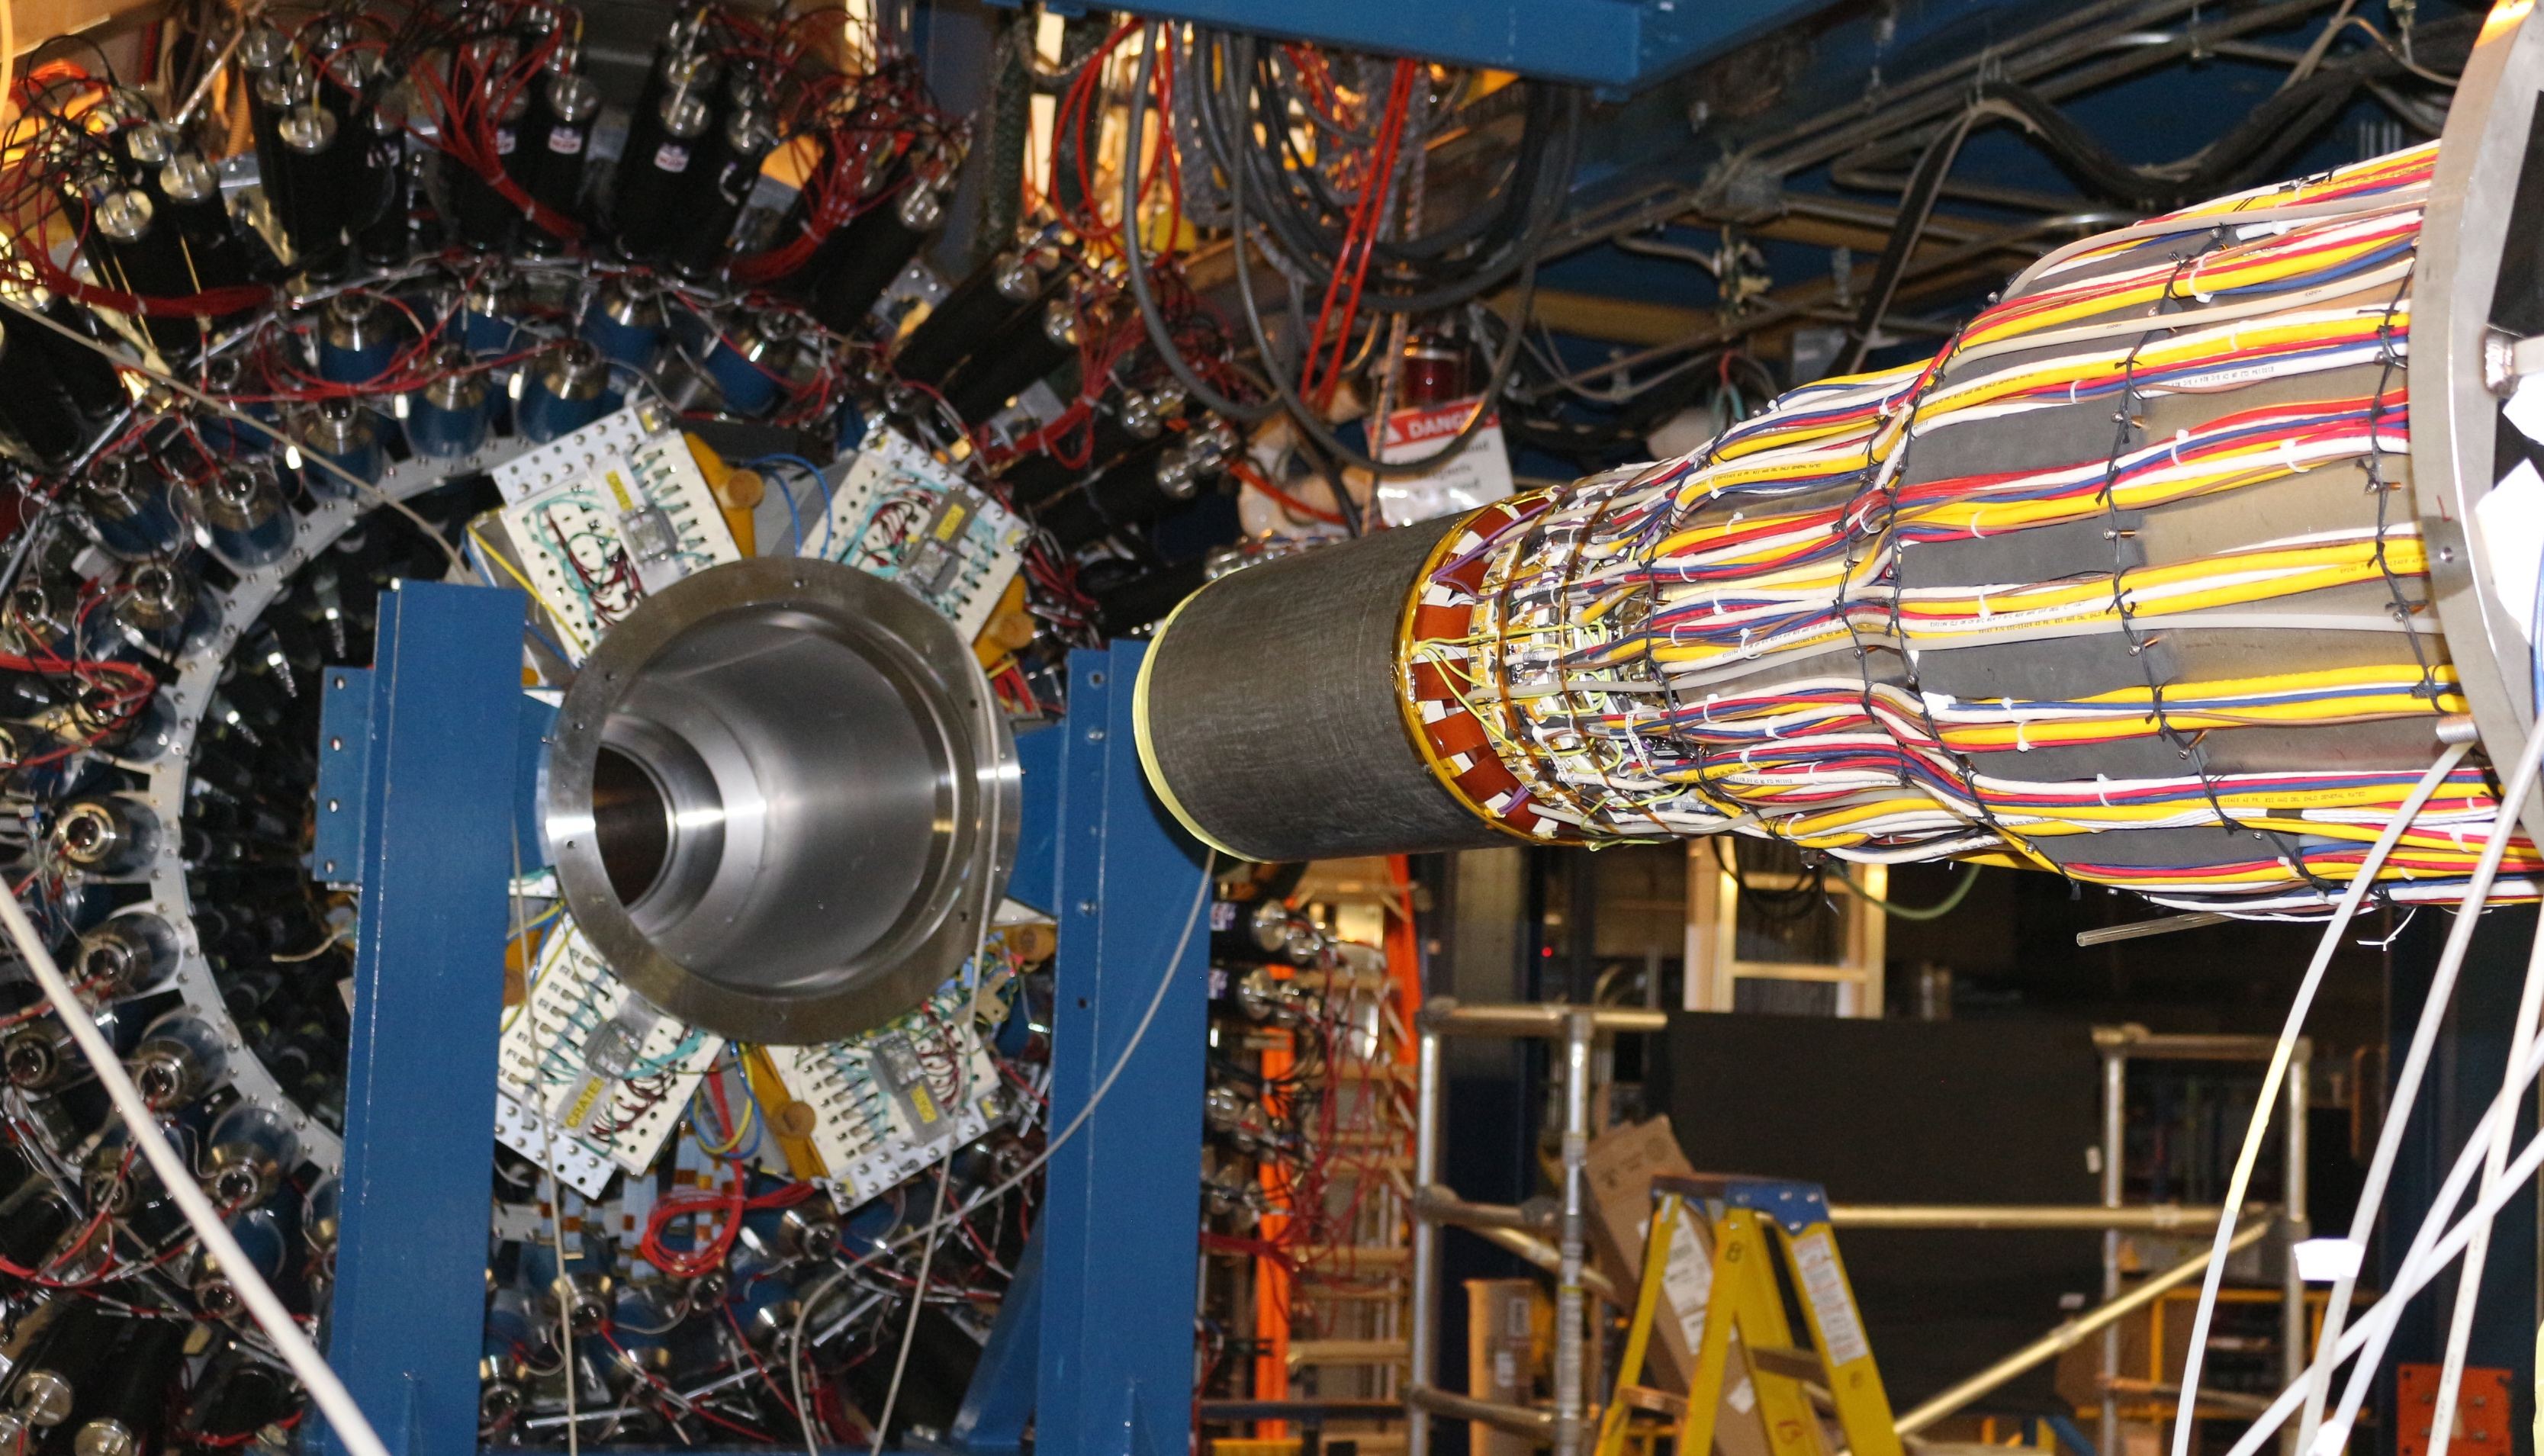
\includegraphics[width=0.5\columnwidth,keepaspectratio]{svt-hall.png}
\caption{SVT detector installed in the experimental hall.}
\label{fig:svt-hall}
\end{figure}

\subsection{Commissioning with cosmic rays}

\begin{figure}[hbt] 
\centering 
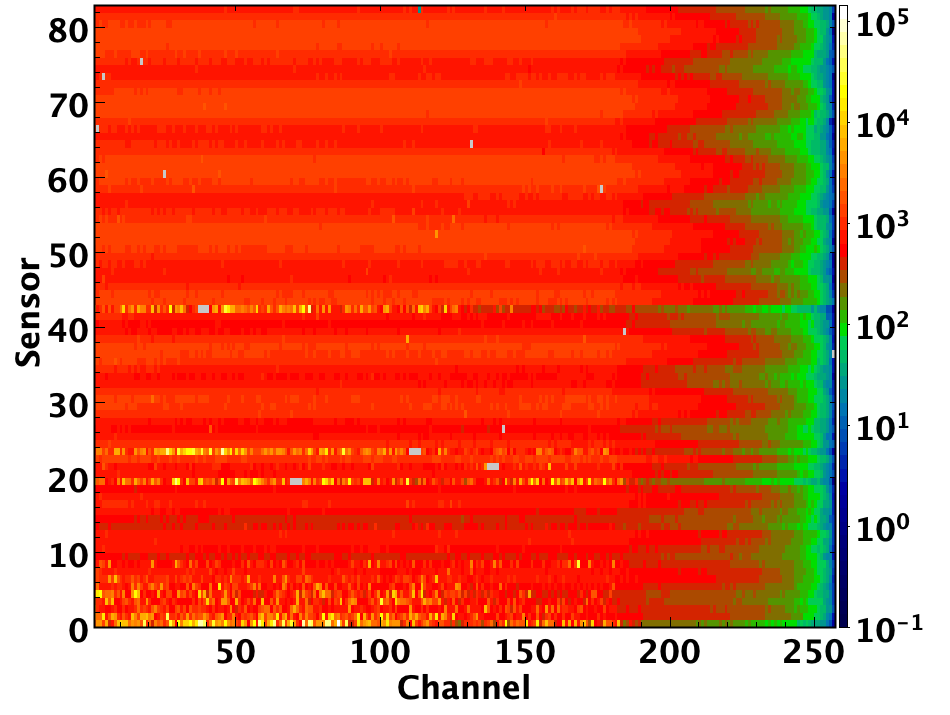
\includegraphics[width=0.5\columnwidth,keepaspectratio]{cosmic-hitmap-svt.png}
\caption{Monitoring SVT hit map during cosmic run.}
\label{fig:cosmic-hitmap-svt}
\end{figure}

Cosmic ray tests of the SVT have been used to test track reconstruction routines for the SVT, as well as establish correct readout, good noise performance, and full response for the entire detector. Cosmic data were taken in the standalone mode using the self triggering feature of the readout in coincidence logic. Angular distribution of the cosmic muons reconstructed in the SVT is shown in Fig.~\ref{fig:track-phi-theta}.

\begin{figure}[hbt] 
\centering 
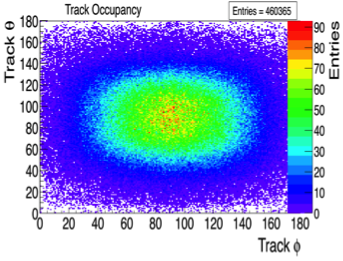
\includegraphics[width=0.5\columnwidth,keepaspectratio]{track-phi-theta.png}
\caption{Angular distribution of the cosmic muons reconstructed in the SVT}
\label{fig:track-phi-theta}
\end{figure}

\subsection{Commissioning with beam}

The impact of the shield on the SVT occupancy is shown in Figure~\ref{fig:hit-occupancy-shielding}. Occupancies in all SVT layers are substantially lower which results in better tracking performance due to reduced combinatorics. The effect of the shield on tracking performance is negligible~\cite{SHIELDNOTE}.

\begin{figure}[hbt] 
\centering 
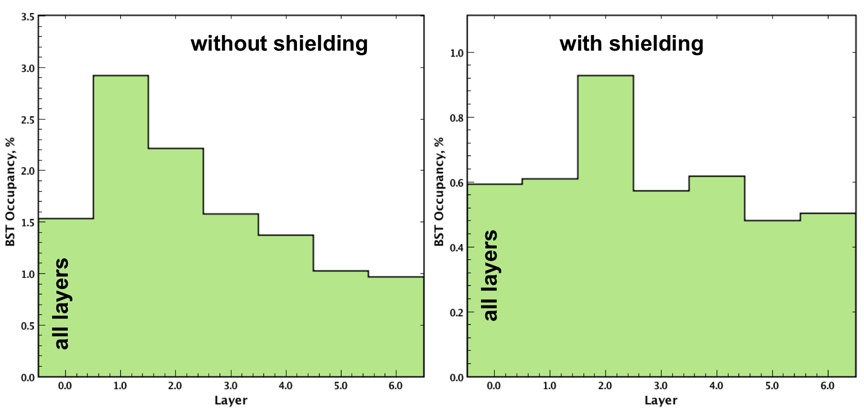
\includegraphics[width=0.5\columnwidth,keepaspectratio]{hit-occupancy-shielding.png}
\caption{Hit occupancies with and without the shield.}
\label{fig:hit-occupancy-shielding}
\end{figure}

%\subsection{Tracking performance, resolution, efficiency}